\section{Input files}
This section of the documentation details the inputs files and conventions that that are necessary to perform sizing. \hydra \spc inputs and outputs are handled using \textbf{yaml} files through the \textbf{pyyaml} package. The yaml input files are converted to \python \spc dictionaries when read, allowing the inputs to be specified in any order. The main dictionaries in \textbf{input.yaml} are \textcolor{red}{\textbf{Sizing}}, \textcolor{red}{\textbf{Configuration}}, \textcolor{red}{\textbf{Mission}} and \textcolor{red}{\textbf{Aircraft}}. All four dictionaries must be present in \textbf{input.yaml}. Two example files are shown below with the \textcolor{red}{\textbf{main dictionary names}} and \blue{sub-dictionary names} highlighted. The two main input files are \textbf{input.yaml} and \textbf{defaults.yaml}.

\subsection{Single main rotor helicopter}
\subsection*{Input file 1: input.yaml}
This input file specifies the mission profile, vehicle configuration, propulsion type and masses of fixed weight groups (e.g., crew, payload, mission equipment). The input file is subdivided into multiple segments, and each input and its units are explained in the following sections. The following input file is used to size a single main rotor/tail rotor helicopter with a mechanical transmission and turboshaft engines. An example single main rotor helicopter is shown in Fig.~\ref{fig:helo}.

\begin{figure}[H]
\begin{center}
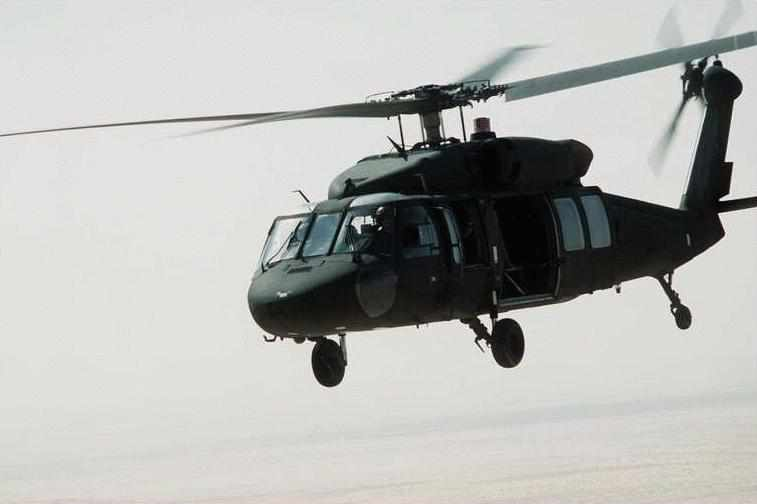
\includegraphics[width=0.5\textwidth]{images/uh60_blackhawk.png}
\caption{UH-60 Blackhawk: single main rotor helicopter}
\label{fig:helo}
\end{center}
\end{figure}

\subsubsection{\red{Sizing} dictionary}
\begin{lstlisting}
<@\textcolor{red}{\textbf{Sizing:}}@>
   <@\blue{Rotors:}@>
      SMR:
         DL:         [10.03]         # lb/ft2
#       radius:     [6.607]          # radius in meters
         Nb:         [4]  
         Vtip:       [213.36] # m/s
         solidity:   [0.1178]
         tip_mach:   [0.95]
         flap_freq:  [1.035]
         cruise_rpm_ratio:  [1.0]
   <@\blue{Fuselage:}@>
      nrotors:         [1]
      liftfraction:    [1.0]
   <@\blue{Powerplant:}@>
      TSEngine: 
         type: `turboshaft'
         num:  2
         redundancy: 0        # how many units can fail, group still works
   <@\blue{Transmission:}@>
      Trans1: 
         type:       `mechanical'
         eta:        0.98
#fidelity options for weight and performance models
   ifea:               False
   use_bemt:           False
\end{lstlisting}

The \red{Sizing} dictionary specifies the values of high-level design variables to use for vehicle sizing. Up to five sub-dictionaries (\blue{Rotor}, \blue{Wings}, \blue{Fuselage}, \blue{Transmission}, and \blue{Powerplant}) and two logical inputs for using higher-fidelity models constitute the sizing dictionary.
\paragraph{\blue{Rotors}}
\blue{Rotors} consists of sub-dictionaries, with each sub-dictionary corresponding to a rotor. In the present example, there is only one rotor that is sized by user-given inputs. The rotor that is sized is the main rotor, called ``SMR'' (Single Main Rotor). The actual name of the rotor can be any string, i.e., \texttt{SMR} is not a keyword, but \texttt{\blue{Rotors}} is a keyword. If neither of these keywords are specified, then the rotor group must be mounted on wings, and its diameter is determined from geometric requirements (largest rotor that fits on all wings that the rotor is mounted on, with adequate rotor-rotor clearance and rotor-fuselage spacing).
\begin{lstlisting}
   <@\blue{Rotors:}@>
      SMR:
         DL:         [10.03]         # lb/ft2
#       radius:     [6.607]          # radius in meters
         Nb:         [4]  
         Vtip:       [213.36] # m/s
         solidity:   [0.1178]
         tip_mach:   [0.95]
         flap_freq:  [1.035]
         cruise_rpm_ratio:  [1.0]
\end{lstlisting}
\noindent ``SMR'' is parameterized using the following \textbf{keywords} shown in Table~\ref{tbl:rotor_keywords}. The last keyword \textcolor{gray}{\textbf{radius}} is grayed out, because it is not used in the present example (the corresponding line in the input file is commented out, indicated by the `\#' symbol). The \textbf{radius} keyword may be specified as an alternate to rotor disk loading. 

\paragraph{\blue{Fuselage}}
The \blue{Fuselage} dictionary is shown below, and the keywords used to define the fuselage are shown in Table~\ref{tbl:fuselage_keywords}.
\begin{lstlisting}
   <@\blue{Fuselage:}@>
      nrotors:         [1]
      liftfraction:    [1.0]
\end{lstlisting}

\begin{center}
  \begin{table}[H]
	\caption{Keywords for sizing a helicopter rotor}
	\label{tbl:rotor_keywords}
    \begin{tabular}{| c | l | c |}
    \hline
    Keyword & Meaning & Value in example \\ 
    \hline
\textbf{DL} & Disk loading & 10.03 lb/ft$^2$ \\
\textbf{Nb} & Number of blades & 4 \\
\textbf{Vtip} & Rotor hover tip speed & 213.36 m/s \\
\textbf{solidity} & Geometric solidity & 0.1178 \\
\textbf{tip\_mach} & Maximum blade tip Mach number & 0.95 \\
\textbf{flap\_freq} & First flap natural frequency in hover & 1.035/rev \\
\textbf{cruise\_rpm\_ratio} & Rotor cruise RPM/hover RPM & 1.0\\
\textcolor{gray}{\textbf{radius}} & \textcolor{gray}{Rotor radius} & \textcolor{gray}{6.607 m} \\
    \hline
  \end{tabular}
\end{table}
\end{center}
%\vspace{-1cm}
\begin{center}
  \begin{table}[H]
	\caption{Keywords for sizing a fuselage}
	\label{tbl:fuselage_keywords}
    \begin{tabular}{| c | l | c |}
    \hline
    Keyword & Meaning & Value in example \\ 
    \hline
\textbf{nrotors} & Number of rotors mounted on this fuselage & 1 \\
\textbf{liftfraction} & Lift fraction carried by fuselage-mounted rotors & 1.0 \\
    \hline
  \end{tabular}
\end{table}
\end{center}

\paragraph{\blue{Powerplant}}
The \blue{Powerplant} definition is shown below. There is only one powerplant group, called `TSEngine' (TurboShaft Engine). 
\begin{lstlisting}
   <@\blue{Powerplant:}@>
      TSEngine: 
         type: `turboshaft'
         num:  2
         redundancy: 0        # how many units can fail, group still works
\end{lstlisting}
Here, `TSEngine' is not a keyword: it is only the name given to the powerplant group, just as `SMR' is the name of the rotor group. This powerplant group is defined using the keywords shown in Table~\ref{tbl:powerplant_keywords}. Here, there are two turboshaft engines, sized so that no engines may fail if adequate power is required in all segments of the sizing mission (excluding margins - specified later in defaults.yaml, Engine parameters ).

\begin{table}[H]
\begin{center}
	\caption{Keywords for sizing a powerplant}
	\label{tbl:powerplant_keywords}
    \begin{tabular}{| c | l | c |}
    \hline
    Keyword & Meaning & Value in example \\ 
    \hline
\textbf{type} & Type of powerplant, character string & `turboshaft' \\
\textbf{num} & Number of engines/units & 2  \\
\textbf{redundancy} & No. of unit failures allowed & 0 \\
    \hline
  \end{tabular}
\end{center}
\end{table}
\vspace{-1.5cm}

\paragraph{\blue{Transmission}}
The \blue{transmission} input block is shown below. There is only one transmission in this conventional helicopter, named `Trans1'. The name of the transmission group (Trans1) is not a keyword, but the attributes of this transmission group are defined using keywords described in Table~\ref{tbl:transmission_keywords}.

\begin{lstlisting}
   <@\blue{Transmission:}@>
      Trans1: 
         type:       `mechanical'
         eta:        0.98
\end{lstlisting}

  \begin{table}[H]
\begin{center}
	\caption{Keywords for sizing a transmission}
	\label{tbl:transmission_keywords}
    \begin{tabular}{| c | l | c |}
    \hline
    Keyword & Meaning & Value in example \\ 
    \hline
\textbf{type} & Type of transmission, character string & `mechanical' \\
\textbf{eta} & Transmission efficiency (power out/power in) & 0.98  \\
    \hline
  \end{tabular}
\end{center}
\end{table}
\vspace{-1.5cm}

\paragraph{High-fidelity model switches}
The keyword \textbf{ifea} is a logical input, used to specify if the FEA-based weight model is to be used in the sizing loop to estimate the airframe structural weight. The other keyword \textbf{use\_bemt} indicates whether the Blade Element Momentum Theory (BEMT) should be used to refine rotor performance estimates in hover (and cruise for prop-rotors). In this example, both options are not enabled. 

\subsubsection{Aircraft \red{Configuration}}
The \red{Configuration} dictionary specifies the associations between rotors, wings (if present), fuselage, transmissions and powerplants (defined in the \red{Sizing} dictionary). This dictionary provides the crucial mapping that specifies where rotors are mounted, and the transmissions connecting various powerplants to the rotor groups. The group names (SMR, Trans1 and TSEngine) are used to specify these connections and size power sources using rotor power required and transmission efficiencies. 

\begin{lstlisting}
<@\red{Configuration:}@>
   <@\blue{Fuselage:}@> `SMR'                 # which rotors are mounted on fuselage
   <@\blue{Rotors:}@>
      SMR: `Trans1'                 # transmission used to power the rotors
   <@\blue{Transmission:}@>                   # powerplant connected to transmissions
      Trans1:                       # transmission group name 
         Powerplant: `TSEngine'     # powerplant group name
         PowerFraction: 1.0         # rated power fraction supplied 
\end{lstlisting}

The various keywords used to associate vehicle components are explained in Table~\ref{tbl:config_smr}. The associations between rotors, fuselages and wings are specified as key-value pairs. The present example is interpreted by \hydra \spc as
\begin{enumerate}
\item The \blue{Fuselage} supports the rotor group called `\texttt{SMR}' 
\item The \blue{Rotors} dictionary specifies that the rotor group \texttt{SMR} draws power through the transmission group `\texttt{Trans1}'
\item The \blue{Transmission} dictionary specifies that the transmission group \texttt{Trans1} draws 100\% of its required power from the powerplant group \texttt{`TSEngine'}.
\end{enumerate}
  \begin{table}[H]
\begin{center}
	\caption{Keywords for defining vehicle configuration}
	\label{tbl:config_smr}
    \begin{tabular}{| c | l | c |}
    \hline
    Keyword & Meaning & Value in example \\ 
    \hline
\textbf{Fuselage} & Specifies rotor mounted on fuselage & `SMR' \\
\textbf{Rotors} & Specifies transmissions powering each rotor group & SMR: `Trans1' \\
\textbf{Transmission} & Sub-dictionaries specify transmission details & `Trans1' \\
\textbf{Powerplant} & Following name specifies associated powerplant & `TSEngine' \\
\textbf{PowerFraction} & Fraction of rated power from `TSEngine' above & 1.0 \\
    \hline
  \end{tabular}
\end{center}
\end{table}
\vspace{-1cm}
\subsubsection{\red{Mission profile}}
The sizing mission profile is specified through several keywords; the meaning of these keywords is explained below, and summarized in Table~\ref{tbl:mission_keywords}. 

The parameter \textbf{nsegments} specifies the number of mission segments. Each segment type can be `hover' or `cruise', specified by the parameter \textbf{flight\_mode}. For hover segments, the duration is specified by the parameter \textbf{time\_seg}. For cruise segments, either the segment duration can be specified, or the \textbf{distance} can be provided as an input and the segment velocity \textbf{cruise\_speed} will be calculated. If the distance is provided as a non-zero input value, the cruise segment duration input is ignored. For climb segments, the start and end altitudes \textbf{start\_altitude}, \textbf{end\_altitude} are specified in meters. 

The parameter \textbf{add\_payload} is used to inform the analysis that the payload has changed at the end of a mission segment (e.g., cargo picked up/dropped off or passenger disembarked/entered the vehicle). The input parameter \textbf{segment\_type} specifies the type of mission segment - `all' indicates the segment is used in day-to-day operations, while `reserve' indicates that the segment is used for sizing, nut not operating cost calculations. The parameter \textbf{sizing\_order} is a list of integers, with zero specifying that the segment is not used for sizing, and a non-zero integer specifying that the segment is used to size a particular component. Usually, the first hover segment and first cruise segment are used for sizing various components. The final line is an optional input specifying the parameter \textbf{fixed\_GTOW}. If this line is present, it instructs the analysis to run sizing in fixed take-off weight mode, and estimate the payload.

\begin{lstlisting}
<@\red{Mission:}@>
   nsegments:          5
   flight_mode:        [ 'hover', 'cruise', 'cruise', 'cruise', 'cruise'] 
   segment_type:       [ 'all',    'all',    'all',    'all',    'all'] 
   time_seg:           [      5,     2.42,     8.23,     84.9,        5] # minutes
   start_altitude:     [ 1219.2,   1219.2,   1828.8,   1828.8,      0.0] # m
   end_altitude:       [ 1219.2,   1828.8,   1828.8,   1828.8,      0.0] # m
   delta_temp_isa:     [ 27.92,    11.88,         0,        0,        0] # deg C
   rate_of_climb:      [      0,   251.86,        0,        0,        0] # m/min
   cruise_speed:       [      0,    85.33,   157.16,   159.03,    70.74] # knots
   add_payload:        [      0,        0,        0,        0,        0] # 
   distance:           [      0,      0.0,    39.93,    416.7,      0.0] # km
   fixed_GTOW:         6454.0               # derive payload for fixed weight
\end{lstlisting}

\begin{center}
  \begin{table}[H]
	\caption{Keywords for defining mission}
	\label{tbl:mission_keywords}
    \begin{tabular}{| c | l | c |}
    \hline
    Keyword & Meaning & Value in example \\ 
    \hline
\textbf{nsegments} & Number of segments in sizing mission & 6 \\
\textbf{flight\_mode} & Specifies type of mission segment & `hover', `cruise' \\
\textbf{time\_seg} & Segment duration in minutes & \textcolor{gray}{--} \\
\textbf{start\_altitude} & Altitude at start of segment (m) & \textcolor{gray}{--} \\
\textbf{end\_altitude} & Altitude at end of segment (m) & \textcolor{gray}{--} \\
\textbf{delta\_temp\_isa} & Temperature offset at sea level (C) & \textcolor{gray}{--} \\
\textbf{rate\_of\_climb} & Vehicle rate of climb in the segment (m/min) & \textcolor{gray}{--} \\
\textbf{cruise\_speed} & Horizontal speed parallel to ground (knots) & \textcolor{gray}{--} \\
\textbf{add\_payload} & Payload added at end of segment (kg) & \textcolor{gray}{--} \\
\textbf{distance} & Horizontal distance covered (km) & \textcolor{gray}{--} \\
\textbf{fixed\_GTOW} & Total weight to hold constant (kg) & \textcolor{gray}{--} \\
     \hline
  \end{tabular}
\end{table}
\end{center}

\subsubsection{\red{Aircraft} details}
The aircraft specification dictionary is show below, and the relevant keywords are summarized in Table~\ref{tbl:aircraft_keywords}. The payload mass, crew mass, common equipment and avionics mass are fixed mass groups, specified in kg. The parameter \textbf{common\_per\_pax} is the mass of equipment that is multiplied by the number of passengers, specified by \textbf{pax\_count}. Based on the number of passengers, additional payload is added internally with the following map: 150 kg for first passenger, 125 kg for next two passengers and 120 kg for the fourth and fifth passengers.
\begin{lstlisting}
<@\red{Aircraft:}@>
   aircraftID: 1
# payload and crew (kg)
   mass_payload:      1134.0
   common_equipment:  1412.0    # fixed values from ndarc output
   pax_count:         0 
   common_per_pax:    0.0
   avionics:          0
\end{lstlisting}
\begin{center}
  \begin{table}[H]
	\caption{Keywords for defining miscellaneous details}
	\label{tbl:aircraft_keywords}
    \begin{tabular}{| c | l | c |}
    \hline
    Keyword & Meaning & Value in example \\ 
    \hline
\textbf{aircraftID} & Flag: helicopters (1) or eVTOL (other) & 1 \\
\textbf{mass\_payload} & Payload mass (kg) & 1134 \\
\textbf{common\_equipment} & Mission equipment mass (kg) & 1412 \\
\textbf{pax\_count} & Number of passengers with bags & 0 \\
\textbf{common\_per\_pax} & Mission equipment per passenger (kg) & 0 \\
\textbf{avionics} & Avionics group mass (kg) & 0 \\
     \hline
  \end{tabular}
\end{table}
\end{center}
\vspace{-2cm}
\subsection*{Input file 2: defaults.yaml}
This input file contains the sizing constraints, motor efficiencies, powerplant details, calibration factors for empirical/reduced-order weight and peformance models and cost models. Also included are ``technology factors'', i.e., multipliers applied to weight predictions for each component. The file is too large to be printed verbatim as a whole unit; instead the text is subdivided into dictionary-sized segments, and each dictionary in this input file is detailed below. 
\vspace{-0.5cm}
\subsubsection{\red{Sizing} constraints}
\vspace{-0.5cm}
\begin{lstlisting}
<@\red{Sizing:}@>
   <@\blue{Constraints:}@>
      max_rotor_radius:    30.0 
      max_gtow: 20000.0
      max_ct_sigma: 0.14
\end{lstlisting}

\begin{center}
  \begin{table}[H]
	\caption{Keywords for defining sizing constraints}
	\label{tbl:constraint_keywords}
    \begin{tabular}{| c | l | c |}
    \hline
    Keyword & Meaning & Value in example \\ 
    \hline
\textbf{max\_rotor\_radius} & Upper limit on hover d-value (meters) & 30  \\
\textbf{max\_gtow} & Upper limit on take-off mass  (kg) & 20000 \\
\textbf{max\_ct\_sigma} & Upper limit on hover blade loading & 0.14 \\
     \hline
  \end{tabular}
\end{table}
\end{center}
\vspace{-1cm}
\blue{Constraints} used to size the vehicle are specified in this dictionary. The first parameter \textbf{max\_rotor\_radius} is the maximum rotor radius (for single main rotor helicopters) or the maximum vehicle footprint (for eVTOL). The parameter \textbf{max\_ct\_sigma} is the upper limit on rotor blade loading in hover. Finally, \textbf{max\_gtow} is the upper limit on take-off mass imposed for the vehicle. These constraints are imposed during optimization as well as iterative sizing. If any of these three constraints are violated during fixed-point iterations, the sizing loop is terminated and the design is marked ``invalid''.

\subsubsection{\red{Empirical} parameters}
This dictionary contains several sub-dictionaries, each of which are detailed below. A sample dictionary is broken into sub-dictionaries and explained below.

\paragraph{\blue{Engines}}
For fuel-burning engines, the \blue{Engines} dictionary is used to set relevant high-level properties of turboshaft engines, summarized in Table~\ref{tbl:turboshaft_keywords}. 
\begin{lstlisting}
   <@\blue{Engines:}@>
      powerHoverAccs : 0.01 # percent of total power for accessories
      effHoverPower  : 1.00 # hover power efficiencies
      loss_filter    : 0.00
      frac_install   : 1.05  # installation losses
   # power lapse rates with density, temperature and installed fractions
      KD_mrp: 1.1132
      KD_irp: 1.1379
      KD_mcp: 1.1000
      KT_mrp: 2.1445
      KT_irp: 2.2248
      KT_mcp: 2.2407
      fracPowerIdle: 0.2
      fracPowerIRP : 0.932
      fracPowerMCP : 1.0
\end{lstlisting}

  \begin{table}[H]
\begin{center}
	\caption{Keywords for defining turboshaft engine properties}
	\label{tbl:turboshaft_keywords}
    \begin{tabular}{| c | l | c |}
    \hline
    Keyword & Meaning & Value in example \\ 
    \hline
\textbf{powerHoverAccs} & Power for accessories (fraction of rotor power) & 0.01  \\
\textbf{effHoverPower} & Additional rotor efficiency knockdowns & 1 \\
\textbf{loss\_filter} & Engine power loss fraction from intake filters & 0.00 \\
\textbf{frac\_install} & Engine installation power loss (fraction) & 0.00 \\
\textbf{KD\_MRP} & Max. rated power lapse rate w/ density & 1.1132\\
\textbf{KD\_IRP} & Intermediate power lapse rate w/ density & 1.1379\\
\textbf{KD\_MCP} & Max continuous power lapse rate w/ density & 1.1000\\
\textbf{KT\_MRP} & Max rated power lapse rate w/ temperature & 2.1445\\
\textbf{KT\_IRP} & IRP lapse rate w/ temperature & 2.2248\\
\textbf{KT\_MCP} & MCP lapse rate w/ temperature& 2.2407\\
\textbf{fracPowerIdle} & Idle power to installed power & 0.2 \\
\textbf{fracPowerIRP} & Intermediate power to installed power & 0.932\\
\textbf{fracPowerMCP} & MCP/installed power & 1.0\\
     \hline
  \end{tabular}
\end{center}
\end{table}
\vspace{-1cm}
\paragraph{\blue{Aerodynamics}}
The \blue{aerodynamics} dictionary is used to specify parameters for calculating rotor hover efficiency, interference losses and body drag. A sample dictionary is shown below, and the keywords are summarized in Table~\ref{tbl:aero_keywords}. 
\begin{enumerate}
\item \textbf{hover\_dwld\_factor} is the additional fraction of nominal rotor lift share that the rotor has to produce in hover to overcome vertical down-load due to the rotor wake impinging on the structure of the vehicle
\item \textbf{cd0} is the average profile drag coefficient of the rotor blade airfoil section
\item \textbf{induced\_power\_factor} accounts for non-ideal induced losses
\item \textbf{FM} is the rotor hover figure of merit. If the hover figure of merit is given as non-zero, then \textbf{FM} is used to estimate rotor shaft power in hover. If the value of figure of merit is given as zero, then the profile drag coefficient and induced power factor are used to estimate rotor hover power. 
\item \textbf{kint} is the rotor power scaling factor to account for interference losses. 
\item \textbf{hover\_thrust} is a character input that ignores the calculated rotor lift share, and distributes the hover thrust equally across all rotors in the system. %This input is primarily present for backward-compatibility, and should not be used extensively except for debugging.
\end{enumerate}
\noindent The empirical parameters used to model wing performance are the Oswald efficiency factor \textbf{oswald} (additional induced drag for non-elliptical span loading) and the mean profile drag coefficient \textbf{cd0}. The efficiencies of dedicated cruise propellers and prop-rotors in cruise is quantified by the \textbf{Propeller} parameter \textbf{eta}. Finally, the scaling factor to estimate body drag from weight using a weight-drag trendline is the parameter \textbf{flat\_plate\_factor}. If this input is zero, then the analysis uses a component drag build-up to estimate parasitic drag.
\begin{lstlisting}
   <@\blue{Aerodynamics:}@>
      Rotors:
         hover_dwld_factor:    0.045
         cd0:                  0.011
         induced_power_factor: 1.15
         kint:                 1.0
         FM:                   0.75
      Body:
         flat_plate_factor: 4.0
\end{lstlisting}

\begin{center}
  \begin{table}[H]
	\caption{Keywords for defining rotor performance and body drag}
	\label{tbl:aero_keywords}
    \begin{tabular}{| c | l | c |}
    \hline
    Keyword & Meaning & Value in example \\ 
    \hline
\textbf{hover\_dwld\_factor} & Vertical down-load/rotor lift in hover & 0.045  \\
\textbf{cd0} & Blade airfoil profile drag coefficient & 0.011  \\
\textbf{induced\_power\_factor} & Total induced power/ideal power & 1.15 \\
\textbf{kint} & Rotor interference loss factor & 1.0 \\
\textbf{FM} & Rotor hover figure of merit & 0.75 \\
\textbf{flat\_plate\_factor} & Coefficient in drag-weight trends & 4.0 \\
     \hline
  \end{tabular}
\end{table}
\end{center}
\paragraph{\blue{Technology factors}}
The term technology factor refers to scaling factors (``multipliers'') used to increase or decrease component empty weights to account for improvements in lightweight manufacturing. If these factors are not entered, default values of 1  are automatically assigned. The relevant keywords are summarized in Table~\ref{tbl:techfac_keywords}.
\begin{center}
  \begin{table}[H]
	\caption{Keywords for defining technology factors}
	\label{tbl:techfac_keywords}
    \begin{tabular}{| c | l | c |}
    \hline
    Keyword & Group weight modified & Value in example \\ 
    \hline
\textbf{landing\_gear} & Alighting gear &  0.3523 \\
\textbf{emergency\_sys} & Parachute for eVTOLs & 0 \\
\textcolor{gray}{\textbf{rotor}} & Rotor blades, hubs, collective actuator & (assumed 1) \\
\textcolor{gray}{\textbf{empennage}} & Horizontal/vertical stabilizers & (assumed 1) \\
\textcolor{gray}{\textbf{fuselage}} & Fuselage & (assumed 1) \\
\textcolor{gray}{\textbf{fuel\_system}} & Fuel handling: tanks and pumps & (assumed 1) \\
\textcolor{gray}{\textbf{drive\_system}} & Transmissions & (assumed 1) \\
\textcolor{gray}{\textbf{flight\_control}} & Flight controls and hydraulics& (assumed 1) \\
\textcolor{gray}{\textbf{powerplant}} & Engines and batteries & (assumed 1) \\
\textcolor{gray}{\textbf{fuel}} & Fuel & (assumed 1) \\
\textcolor{gray}{\textbf{battery}} & Batteries & (assumed 1) \\
     \hline
  \end{tabular}
\end{table}
\end{center}
\vspace{-1cm}
The sample input block is shown below:
\begin{lstlisting}
   <@\blue{Tech\_factors:}@>
      Weight_scaling:
         landing_gear:     0.3523      #  
         emergency_sys:    0.0         # group absent
\end{lstlisting}

\subsection{All-electric tandem tilt-wing}
An example all-electric tandem tilt-wing is shown in Fig.~\ref{fig:vahana}. This aircraft incorporates two lifting wings, with four rotors mounted on each wing. Tilt actuators allow the wings (and therefore the rotors mounted on these wings) to tilt from a vertical orientation in hover to a horizontal orientation in cruise. The example shown in this document is a modified simplification of Vahana, i.e., it is not identical to the aircraft shown in Fig.~\ref{fig:vahana}. In this the example, both wings are assumed to be identical. All 8 rotors are also assumed to be identical. 

\begin{figure}[H]
\begin{center}
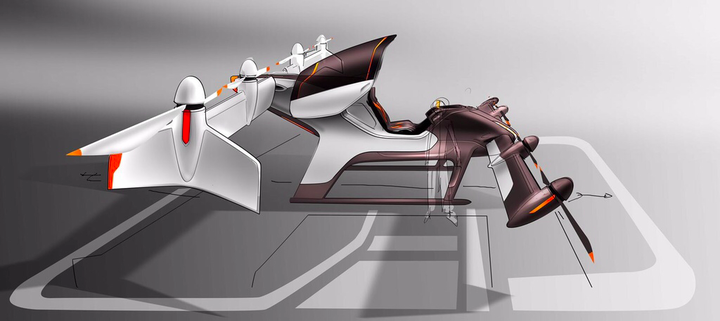
\includegraphics[width=\textwidth]{images/vahana_picture.png}
\caption{Vahana all-electric tandem tilt-wing with 8 rotors}
\label{fig:vahana}
\end{center}
\end{figure}

For the all-electric configuration, the input files are slightly different from the corresponding files for the conventional helicopter. An additional \red{Wings} dictionary is specified, and the propulsion architecture definition is also modified to reflect the new system. 
\subsection*{Input file 1: input.yaml}

\subsubsection{\red{Sizing}}
This dictionary specifies the values of high-level design variables to use for sizing the vehicle. For this vehicle type, \blue{Rotors}, \blue{Wings}, \blue{Fuselage}, \blue{Powerplant} and \blue{Transmission} are all defined and linked with the \red{Configuration} dictionary.

\paragraph{\blue{Rotors}}
The \blue{Rotor} sub-dictionary is shown below. Here, the number of inputs are far fewer than those required to size a helicopter rotor, for several reasons. The blade first flap natural frequency is not specified for eVTOLs, because rotor dynamics is no longer a key driver for blade sizing - sizing for strength automatically results in a very stiff design at the scales of interest. Additionally, neither disk loading nor rotor radius are specified, and so the wing-mounted rotors are automatically sized to ensure that the maximum possible disk area is achieved. Finally, the tip speed is markedly lower than that of a conventional helicopter's rotor, to reduce noise. This input value automatically guarantees that the advancing blade tip mach number in cruise is sufficiently low as to ensure almost zero compressibility drag. By not specifying the cruise rotor speed, a default value of 50\% hover tip speed is assigned. 

\begin{lstlisting}
   <@\blue{Rotors:}@>
      All_rotors:
      All_rotors:
         Nb:         [3]                      # per rotor
         Vtip:       [170]                    # hover tip speed, m/s
         ctsigma:    [0.139]
\end{lstlisting}
This definition shows that there is one rotor group used in the vehicle called `All\_rotors', with three design variables to size rotors in this group:
\begin{enumerate}
\item Number of blades per rotor \textbf{Nb} = 3
\item Tip speed \textbf{Vtip} = 170 m/s
\item Hover blade loading \textbf{ctsigma} = 0.139
\end{enumerate}
For the variable-RPM rotors used in eVTOLs, additional thrust can be achieved by changing the rotor speeds at the same blade loading. Therefore, the strict upper limits of $C_T/\sigma$ - usually observed in conventional helicopters with constant-speed rotors - can be relaxed for eVTOLs. 

\paragraph*{Rotor sizing rules}
If the rotor disk loading in hover is not specified (keyword \textbf{DL}, lb/sq.ft) and the rotor radius (keyword \textbf{radius}, meters) is also not specified, the rotor is assumed to be mounted on a wing, and the size is set based on wing span (calculated in fixed wing sizing) and rotor tip clearance (specified in \textbf{defaults.yaml}). After calculating rotor radius, the tip speed is used to identify the mean \textbf{rotor blade chord}. If the rotor geometric solidity (keyword \textbf{solidity}) is specified, then the hover blade loading is calculated. Otherwise, the the hover blade loading (keyword \textbf{ctsigma}) must be specified, and the geometric solidity is calculated. Some additional inputs are rotor cruise RPM to hover RPM ratio (keyword \textbf{RPM\_ratio}), and first flap frequency in hover (keyword \textbf{fl\_freq}). If these inputs are not specified, then default values of $\Omega_C/\Omega_H$ = 0.5 and $\nu_\beta$=1.1/rev are assumed. 

\paragraph{\blue{Wings}}
The \blue{Wings} dictionary consists of sub-dictionaries, with each sub-dictionary corresponding to a fixed wing group. Several instances of this fixed wing unit may exist on the vehicle; this detail is specified by the parameter \textbf{nwing}. In the example shown above, the \blue{Wings} dictionary is shown below, and the relevant keywords are summarized in Table~\ref{tbl:wing_keywords}.

\begin{lstlisting}
   <@\blue{Wings:}@>
      Main_wing:
         nwing:            [2]
         aspectratio:      [3,4,5,6,7,8] 
         cl:               [0.3,0.4,0.5,0.6,0.7]
         liftfraction:     [1]
         nrotors:          [4]
\end{lstlisting}

\begin{center}
  \begin{table}[H]
	\caption{Keywords for defining wing parameters}
	\label{tbl:wing_keywords}
    \begin{tabular}{| c | l | c |}
    \hline
    Keyword & Meaning & Value in example \\ 
    \hline
\textbf{nwing} & Number of fixed wings in this set &  2 \\
\textbf{aspectratio} & Wing geometric aspect ratio & [3, 4, ..] \\
\textbf{cl} & Wing lift coefficient in cruise & [0.3, 0.4, ..] \\
\textbf{liftfraction} & Weight fraction in cruise carried by this wing set & 1 \\
\textbf{nrotors} & Number of rotors mounted on each wing & 4 \\
     \hline
  \end{tabular}
\end{table}
\end{center}
\vspace{-1cm}

This input specifies one fixed wing group called ``Main\_wing'', of which there are \textbf{nwing}=2 identical units. The name ``Main\_wing'' is not a keyword - it is a character string that is used to refer to the set of wings defined using \textbf{keywords}, and build associations with rotor groups through the \red{Configuration} dictionary. The parameter \textbf{aspectratio} is the wing aspect ratio $b^2/S_{\rm wing}$, \textbf{cl} is the wing cruise lift coefficient and \textbf{liftfraction} is the fraction of vehicle weight carried by the the \textbf{nwing} units in this wing group during cruise. Finally, the parameter \textbf{nrotors} specifies the number of rotors mounted on a wing of this group. Here, 4 rotors are mounted on each wing in this group. Each input parameter can be specified as a single value or list of values to use for sizing.

\paragraph{\blue{Fuselage}}
The fuselage input dictionary for the tilt-wing is shown below. The dictionary specifies that the fuselage does not directly support any rotors, and that it is responsible for carrying no cruise lift. 
\begin{lstlisting}
   <@\blue{Fuselage:}@>
      nrotors:      [0]
      liftfraction: [0.0]
\end{lstlisting}

\paragraph{\blue{Powerplant}}
The source of power for the all-electric aircraft is a Lithium-ion battery, defined as shown below. The name \texttt{`BatteryPack'} is not a keyword - it is only the name of the powerplant group that supplies energy to the system. The keyword \textbf{type} is defined as `battery' to indicate the use of a Lithium-ion pack. The details for the battery cells and pack assembly are provided in \textbf{defaults.yaml}.

\begin{lstlisting}
   <@\blue{Powerplant:}@>
      BatteryPack: 
         type: `battery'
         num:  1
         redundancy: 0        
\end{lstlisting}

\paragraph{\blue{Transmission}}
In this aircraft, there is a single electric transmission, indicated by the keyword \textbf{type} defined as \texttt{`electric'} below. The transmission efficiency is 1, i.e., 100\% of the energy is transmitted without losses (usually 0.98, here shown as 1 for illustrative purposes). Additionally, motor efficiencies in hover and cruise are defined through the keywords \textbf{hover\_efficiency} and \textbf{cruise\_efficiency}. These keywords will be ignored if a higher-fidelity motor model is integrated into the sizing loop (future expansions).

\begin{lstlisting}
   <@\blue{Transmission:}@>
      ElTrans: 
         type:      `electric'
         eta:           1.00
         redundancy:    1.0   
         Motors:
            hover_efficiency: 0.90
            cruise_efficiency: 0.85
\end{lstlisting}

\paragraph{High-fidelity model switches}
The parameter \textbf{ifea} is a logical input, used to specify if the FEA-based weight model is to be used in the sizing loop to estimate the airframe structural weight. The other parameter \textbf{use\_bemt} indicates whether the Blade Element Momentum Theory (BEMT) should be used to refine rotor performance estimates in hover (and cruise for prop-rotors). In this example, both options are not enabled. 

\subsubsection{Aircraft \red{Configuration}}
The vehicle configuration details the association of rotors, wings, transmissions and powerplants. The \blue{Wings} dictionary shows that the wing group called `Main\_wing' supports rotors belonging to the group `All\_rotors'. The \blue{Rotors} dictionary shows that the rotor group `All\_rotors' draws power through the transmission group `ElTrans'. The \blue{Transmission} dictionary indicates that the transmission called `ElTrans' draws all of its power (\textbf{PowerFraction}=1.0) from `BatteryPack'. Each of these building blocks have been defined in the \red{Sizing} dictionary; the \red{Configuration} dictionary is used to create associations between these components. 

For electric transmissions, the analysis automatically sizes the drive motors based on all rotor groups that draw power through a given transmission.

\begin{lstlisting}
<@\textcolor{red}{\textbf{Configuration:}}@>
   <@\blue{Wings:}@>
      Main_wing:     `All_rotors'   # whichrotor group to mount on this wing 
   <@\blue{Rotors:}@>
      All_rotors:    `ElTrans'      # transmission used to power the rotors
   <@\blue{Transmission:}@>                   
      ElTrans:                        # transmission group name 
         Powerplant: `BatteryPack'  # connected powerplant group name
         PowerFraction: 1.0           # rated power fraction supplied 
\end{lstlisting}

\subsubsection*{Configuration mapping rules}
At present, multiple rotors from the same group may be mounted on wings or fuselages. One powerplant may supply energy to multiple transmissions, but  each rotor group may draw power from only one transmission group. However, one transmission group may supply power to multiple rotor groups. Work is ongoing to release advanced features with hybrid powerplants with heterogeneous power sources. 

\subsubsection{\red{Mission profile}}
The mission profile from \textbf{input.yaml} is show below. This input does not require any modification for all-electric vehicles, because it does not depend on the configuration.
\begin{lstlisting}
<@\textcolor{red}{\textbf{Mission:}}@>
   nsegments:          4
   flight_mode:        ['hover','cruise', 'cruise','hover'   ]
   time_seg:           [    1.5,       0,        0,    1.5   ]
   start_altitude:     [    0.0,    00.0,        0,      0   ] # m
   end_altitude:       [    0.0,     0.0,        0,      0   ] # m
   delta_temp_isa:     [    0.0,     0.0,        0,      0   ] # centrigrade
   rate_of_climb:      [      0,       0,        0,      0   ] # m/min
   cruise_speed:       [      0,      98,       98,      0   ] # knots
   distance:           [      0,      50,       15,      0   ] # in km
   add_payload:        [      0,       0,        0,      0   ] # dropped payload 
   segment_type:       [  `all',   `all',`reserve',   `all'  ] # 
   sizing_order:       [      1,       2,        0,      0   ] # order of sizing
\end{lstlisting}

\pagebreak
\subsubsection{\red{Aircraft}}

The aircraft specification dictionary is shown below. This input block also has identical keywords compared to the single main rotor helicopter, because it does not depend on the configuration (only the mission).

\begin{lstlisting}
<@\textcolor{red}{\textbf{Aircraft:}}@>
Aircraft:
   aircraftID: 2
   mass_payload:     345.0       # 250 kg payload + 70 kg margin
   mass_crew:         0 
   avionics:         79.2
   common_equipment: 24.0        # HVAC systems - common for all PAX
   common_per_pax:   00.0
   pax_count:         0          # number of passengers 
\end{lstlisting}

\subsection*{Input file 2: defaults.yaml}
This input file contains the sizing constraints, powerplant details, calibration factors for empirical/reduced-order weight and performance models and cost models. Also included are ``technology factors'', i.e., multipliers applied to weight predictions for each component. The file is too large to be printed verbatim as a whole unit; instead the text is subdivided into dictionary-sized chunks, and each dictionary in this input file is detailed below.

\subsubsection{\red{Sizing} dictionary}
\begin{lstlisting}
<@\red{Sizing:}@>
   <@\blue{Constraints:}@>
      max_rotor_radius:    14.01 # m
      max_ct_sigma    :     0.14
      max_gtow        :  5000.0 # kg
\end{lstlisting}

\blue{Constraints} used to size the vehicle are specified in this dictionary. The first parameter \textbf{max\_rotor\_radius} is the maximum rotor radius (for single main rotor helicopters) or the maximum vehicle footprint (for eVTOL). The parameter \textbf{max\_ct\_sigma} is the upper limit on rotor blade loading in hover. Finally, \textbf{max\_gtow} is the upper limit on take-off mass imposed for the vehicle. These constraints are imposed during optimization as well as iterative sizing. If any of these three constraints are violated during fixed-point iterations, the sizing loop is terminated and the design is marked ``invalid''.

\subsubsection{\red{Empirical} parameters}
This dictionary contains several sub-dictionaries, each of which are detailed below. A sample dictionary is broken into sub-dictionaries and explained below, and the keywords are summarized in Table~\ref{tbl:battery_keywords}.

\paragraph{\blue{Battery}}
The \blue{battery} sub-dictionary features parameters to model individual cells, as well as the battery pack. The cell parameters are \textbf{sp\_energy} (maximum rated energy stored per unit cell mass), \textbf{Tmax} (maximum rated cell temperature), \textbf{energy\_vol} (rated energy per unit cell volume) and \textbf{volume} (unit cell volume in liters).

\begin{lstlisting}
   <@\blue{Battery:}@>
      Cell:
         sp_energy:   240.0      # measured in W-hr/kg
         Tmax:         70.0      # max cell temperature, deg C
         energy_vol:  632.0      # energy density, Watt-hours/liter
         volume:        0.01708  # volume of a cell unit, liters
      Pack:
         SOH:           0.8      # state of health; 0 = gone; 1 = brand new
         DOD_min:       0.075    # minimum depth of discharge;
         integ_fac:     0.75     # battery pack integration factor for mass 
         vol_fac:       0.3      # battery volume integration factor 
      Force_sizing:     `energy' # ignore cell count or temperature effects      
\end{lstlisting}
The battery pack is quantified by the following parameters
\begin{enumerate}
\item State of health \textbf{SOH} - the maximum energy that can be stored in the pack, as a fraction of its rated energy. This parameter is usually less than unity because charge/discharge cycling of cells results in reduced energy storage capacity.
\item Minimum depth of discharge \textbf{DOD\_min} - the minimum energy capacity that the pack must retain to avoid permanent set and reduced energy capacity in individual cells. 
\item Pack mass integration factor \textbf{integ\_fac} - the ratio of battery cell mass to pack mass, to account for the battery casing and power management systems.
\item Pack volume factor \textbf{vol\_fac} - the ratio of cell mass to battery pack mass, to account for additional components introduced by the mass integration factor, as well as clearances for cell cooling.
\item Finally, the battery sizing option \textbf{Force\_sizing} is a string input that directs the battery sizing module to ignores thermal effects and pack voltage constraints; if this input is present, only energy-based sizing is performed.
\end{enumerate}

\begin{center}
  \begin{table}[H]
	\caption{Keywords for defining battery parameters}
	\label{tbl:battery_keywords}
    \begin{tabular}{| c | l | c |}
    \hline
    Keyword & Meaning & Value in example \\ 
    \hline
\textbf{Cell} & Indented entries pertain to cell properties &  -- \\
\textbf{sp\_energy} & Specific energy of a cell (Watt-hr/kg) &  -- \\
\textbf{Tmax} & Maximum cell temperature (deg C) & 70.0 \\
\textbf{energy\_vol} & Cell energy per unit volume (Watt-hr/liter) & 632.0 \\
\textbf{volume} & Volume of cell unit (liters) & 0.01708 \\
\textbf{Pack} & Indented entries pertain to pack properties &  \\
\textbf{SOH} & Average cell state of health (0 to 1) & 0.8 \\
\textbf{DOD\_min} & Minimum depth of discharge allowed (0 to 1) & 0.075 \\
\textbf{integ\_fac} & Mass of cells / mass of pack & 0.75 \\
\textbf{vol\_fac} & Volume of cells / volume of pack & 0.3 \\
\textbf{Force\_sizing} & String input to choose type of sizing & `energy' \\
     \hline
  \end{tabular}
\end{table}
\end{center}
\vspace{-1cm}

\paragraph{\blue{Aerodynamics}}
The \blue{aerodynamics} dictionary is used to specify rotor hover and cruise efficiencies, interference losses, wing efficiencies and body drag. A sample dictionary is shown below.

\begin{lstlisting}
   <@\blue{Aerodynamics:}@>
      Rotors:
         hover_dwld_factor:    0.015
         cd0:                  0.012
         induced_power_factor: 1.18
         FM:                   0.75
         kint:                 1.02
         hover_thrust:         `equal'
      Wings:
         oswald:            0.8
         cd0:               0.014
      Propellers:
         eta:               0.85
      Body:
         flat_plate_factor: 0.88       # means use drag build-up model
\end{lstlisting}

The sub-dictionaries for Rotors, Propellers and Body have been described in the previous section and are not repeated here. The empirical parameters used to model Wing performance are the Oswald efficiency factor \textbf{oswald} (quantifies additional induced drag for non-elliptical span loading) and the mean profile drag coefficient \textbf{cd0}, summarized in Table~\ref{tbl:wing_aero_keywords}. 

\begin{center}
  \begin{table}[H]
	\caption{Keywords for defining wing performance parameters}
	\label{tbl:wing_aero_keywords}
    \begin{tabular}{| c | l | c |}
    \hline
    Keyword & Meaning & Value in example \\ 
    \hline
\textbf{oswald} & Oswald efficiency factor &  0.8 \\
\textbf{cd0} &  Wing airfoil section profile drag coefficient & 0.014 \\
     \hline
  \end{tabular}
\end{table}
\end{center}
\vspace{-2cm}

\begin{center}
  \begin{table}[h]
	\caption{Keywords for defining geometric parameters}
	\label{tbl:geometry_keywords}
    \begin{tabular}{| c | l | c |}
    \hline
    Keyword & Meaning & Value in example \\ 
    \hline
\textbf{fuselage\_width} & Fuselage equivalent diameter (m) &  1.0 \\
\textbf{fuselage\_length} &  Fuselage length (m) & 7.0 \\
\textbf{clearance} &  Rotor tip clearance/radius & 7.0 \\
     \hline
  \end{tabular}
\end{table}
\end{center}
\vspace{-2cm}
\paragraph{\blue{Geometry}}
\begin{lstlisting}
   <@\blue{Geometry:}@>
      fuselage_width:    1.00          # fuselage width in meters
      fuselage_length:   7.00          # fuselage length in meters
      clearance:         0.15          # rotor tip clearance / radius ratio
\end{lstlisting}
The three geometry parameters used for sizing are the fuselage width at the widest point \textbf{fuselage\_width} (meters), airframe length \textbf{fuselage\_length} (meters) and the rotor clearance parameters \textbf{clearance}. This final parameter is the in-plane clearance between a rotor plane and other rotor planes/vehicle fuselage. The geometry parameters are summarized in Table~\ref{tbl:geometry_keywords}.

\paragraph{\blue{Technology factors}}
The term technology factor refers to scaling factors (``multipliers'') used to increase or decrease component empty weights to account for improvements in lightweight manufacturing. A sample dictionary is shown below. In the present case, the wing mass is scaled to 90\% of the predicted value, landing gear is scaled to 40\% of the model prediction and anti-icing group is neglected.
\begin{lstlisting}
   <@\blue{Tech\_factors:}@>
      Weight_scaling:
         wing:             0.9          # wings
         landing_gear:     0.4          #  
         anti_icing:       0.0          # ignored  
\end{lstlisting}

\subsubsection{\red{Acquisition} cost model}

There are two types of costs associated with the rotorcraft that are modeled in \hydra: acquisition cost (component purchase) and operating cost. The dictionary \red{Acquisition} contains three sub-dictionaries: \blue{Fixed\_cost},  \blue{Scaling\_cost} and \blue{Beta\_acq\_factors}. Each of these dictionaries is detailed below with examples.

\paragraph{\blue{Fixed acquisition cost}}
\begin{lstlisting}
<@\red{Acquisition:}@>
   <@\blue{Fixed\_cost:}@>
      sense_avoid:    189817.0            # USD 
      avionics:       145807.0            # USD
      interiors:       45152.0            # USD, air conditioning/heater/HUD
      testing:          6400.0            # USD 
\end{lstlisting}
This sub-dictionary contains inputs for the cost of vehicle components that do not vary with vehicle size. These groups include the sense and avoid system, avionics, interiors and component testing. The keywords for defining acquisition cost parameters are shown in Table~\ref{tbl:acq_cost_keywords}.

\begin{table}[h]
\begin{center}
	\caption{Keywords for defining acquisition cost parameters}
	\label{tbl:acq_cost_keywords}
    \begin{tabular}{| c | l | c |}
    \hline
    Keyword & Meaning & Value in example \\ 
    \hline
\textbf{sense\_avoid} & System purchase cost&  189817.0 \\
\textbf{avionics} & System purchase cost &  145807.0 \\
\textbf{interiors} & System purchase cost &  45152.0 \\
\textbf{testing} & System purchase cost &  6400.0 \\
     \hline
  \end{tabular}
\end{center}
\end{table}

\paragraph{\blue{Scaling\_cost}}
This sub-dictionary contains inputs for the cost of vehicle components that scale with the mass of each component. Several components fall under this category, particularly airframe, wings, landing gear, rotor blade structures, transmission lines and motors. A sample dictionary is shown below, and the relevant keywords are summarized in Table~\ref{tbl:scaling_cost_keywords}.

\begin{lstlisting}
   <@\blue{Scaling\_cost:}@>
      final_assem_line:    90.07          # USD/kg of take-off mass 
      BRS:                 10.885         # USD/kg of take-off mass 
      fuselage:          2807.0           # USD/kg of fuselage weight
      landing_gear:      1725.0           # USD/kg of landing gear strl.  weight
      wing_structure:    3779.1           # USD/kg of wing     structural weight
      motors:            2669.0           # USD/kg of drive motor mass 
      power_dist:          31.0           # USD/kW of installed power
      rotor_blade:      77605.0           # USD/sq.m of plan-form area
      rotor_hub:        14133.0           # USD/kg: hub+collective actuator
      wires:               20.3           # USD/kg of wire weight 
      tilt_actuator:     2868.0           # USD/kg of tilt actuator weight 
      wing_flap:         2619.0           # USD/kg of wing flap/aileron    
\end{lstlisting}

\begin{table}[h]
\begin{center}
	\caption{Keywords for defining cost elements that scale with vehicle properties}
	\label{tbl:scaling_cost_keywords}
    \begin{tabular}{| c | l | c |}
    \hline
    Keyword & Meaning & Value in example \\ 
    \hline
\textbf{final\_assem\_line} & Cost per kg of take-off mass &  90.07 \\
\textbf{BRS} & Cost per kg of emergency parachute mass &  10.885 \\
\textbf{fuselage} & Cost per kg of fuselage mass & 2807.0  \\
\textbf{landing\_gear} & Cost per kg of landing gear mass & 2807.0  \\
\textbf{motors} & Cost per kg of electric motor mass &   2669.0\\
\textbf{power\_dist} & Cost per kg of power distribution system mass & 31.0 \\
\textbf{rotor\_blade} & Cost per kg of rotor blade mass &  77605.0 \\
\textbf{rotor\_hub} & Cost per kg of rotor hub mass &  14133.0 \\
\textbf{wires} & Cost per kg of wire mass &  20.3\\
\textbf{tilt\_actuator} & Cost per kg of tilt actuator mass &  2868.0 \\
\textbf{wing\_flap} & Cost per kg of wing flaps mass &  2619.0 \\
     \hline
  \end{tabular}
\end{center}
\end{table}

\paragraph{\blue{Acquisition cost scaling factors}}
This dictionary deals with cost multipliers that account for reduction of component prices associated with mass-production. A value less than one indicates that the component is less expensive when manufactured in bulk or performed at large scales. The keywords to define these parameters are summarized in Table~\ref{tbl:cost_tech_factors}. 

\begin{lstlisting}
   <@\blue{Beta\_acq\_factors:}@>                    # acquisition cost multipliers 
      sense_avoid:         0.5            
      avionics:            0.75           
      interiors:           1.0            # air conditioning/heater/HUD
      testing:             1.0            
      final_assem_line:    0.5            
      BRS:                 0.75           
      fuselage:            0.2            
      landing_gear:        0.2            
      wing_structure:      0.2            
      motors:              0.2            
      power_dist:          1.0            
      rotor_blade:         0.2            
      rotor_hub:           0.2            
      wires:               1.0            
      tilt_actuators:      0.75           
      wing_flaps:          0.75           
\end{lstlisting}

\begin{table}[H]
\begin{center}
	\caption{Keywords for defining cost scaling factors}
	\label{tbl:cost_tech_factors}
    \begin{tabular}{| c | l | c |}
    \hline
    Keyword & Meaning & Value in example \\ 
    \hline
\textbf{sense\_avoid} & Cost multiplier for sense and avoid system & 0.5 \\
\textbf{avionics} & Cost multiplier for avionics &  0.75 \\
\textbf{interiors} & Cost multiplier for interiors &  1.0 \\
\textbf{testing} & Cost multiplier for final testing &  1.0 \\
\textbf{final\_assem\_line} & Cost multiplier for final assembly line &  0.5 \\
\textbf{BRS} & Cost multiplier for emergency parachute &  0.5 \\
\textbf{fuselage} & Cost multiplier for fuselage structure &  0.5 \\
\textbf{landing\_gear} & Cost multiplier for landing gear structure &  0.5 \\
\textbf{wing\_structure} & Cost multiplier for wing structure&  0.5 \\
\textbf{motors} & Cost multiplier for motors & 0.5 \\
\textbf{power\_dist} & Cost multiplier for power distribution systems &  0.5 \\
\textbf{rotor\_blade} & Cost multiplier for rotor blades &  0.2 \\
\textbf{rotor\_hub} & Cost multiplier for rotor hubs&  0.2 \\
\textbf{wires} & Costmultiplier for wires &  1.0 \\
\textbf{tilt\_actuator} & Cost multiplier for tilt actuators &  0.75 \\
\textbf{wing\_flap} & Cost multiplier for wing flaps &  0.75 \\
     \hline
  \end{tabular}
\end{center}
\end{table}

\subsubsection{\red{Operations}}
Operating costs are of two types: \blue{annual} and \blue{hourly} operating costs. These two components of the operating cost model are specified as sub-dictionaries under \red{Operations}. Additionally, the constants required to obtain \blue{battery} life cycle costs are also specified. Finally, \blue{vertiport} details are also specified and the cost of an eVTOL trip is compared to the cost of using a \blue{taxi} for traveling the same distance. Each of these sub-dictionaries are detailed below.

\paragraph{\blue{Annual} costs}
The sample \blue{Annual} operating cost inputs are shown below, and the relevant keywords are summarized in Table~\ref{tbl:annual_keywords}.
\begin{lstlisting}
<@\red{Operations:}@>
   <@\blue{Annual:}@>
      Flight_hours:        1500              # flight hours per year
      Liability:           22000             # USD liability insurance per year
      Inspection:          7700           # USD, per year
      Insurance_percent:   4.5               # insurance, % of acquisition 
      Depreciation_percent: 10               # % of acquisition cost depr./year
      Pilot:               280500            # USD, pilot cost to company/year
      Training:            9900              # USD, pilot training/year
\end{lstlisting}

The number of flight hours per year (\textbf{Flight\_hours}) is used to calculate the equivalent cost per flight hour from the annual fixed costs incurred in ensuring vehicle airworthiness. The annual costs incurred are \textbf{Liability}, \textbf{Inspection}, insurance and depreciation (specified as a percentage of acquisition cost, \textbf{Insurance\_percent} and \textbf{Depreciation\_percent} respectively). For a piloted vehicle, additional costs are incurred for pilot salary and overhead (\textbf{Pilot}) as well as continuous training (\textbf{Training}). 

\begin{table}[H]
\begin{center}
	\caption{Keywords for defining cost scaling factors}
	\label{tbl:annual_keywords}
    \begin{tabular}{| c | l | c |}
    \hline
    Keyword & Meaning & Value in example \\ 
    \hline
\textbf{Flight\_hours} & Flight hours operated per year & 1500 \\
\textbf{Liability} & Cost for liability insurance per year &  22000\\
\textbf{Inspection} & Cost for annual inspection &  7700\\
\textbf{Insurance\_percent} & Hull insurance as \% of acquisition cost &  4.5\\
\textbf{Depreciation\_percent} & Depreciation as \% of acquisition cost &  10\\
\textbf{Pilot} & Pilot annual salary and benefits &  280500\\
\textbf{Training} & Pilot annual training update cost &  9900\\
     \hline
  \end{tabular}
\end{center}
\end{table}
\vspace{-1cm}

\paragraph{\blue{Hourly} costs}
\noindent This dictionary specifies the maintenance and inspection costs associated with operating an air vehicle. A sample input chunk for \blue{Hourly} costs is shown below, and the keywords are summarized in Table~\ref{tbl:hourly_keywords}. The three elements in this dictionary are 
\begin{enumerate}
\item Frame inspection (\textbf{Frame\_maintenance}): specified as a cost in currency per flight hour
\item Rotor blades, collective actuator and hub inspection (\textbf{Rotor\_inspection}): specified as a cost in currency per flight hour per unit assembly
\item Electric motor inspection (\textbf{Motor\_inspection}): specified as a cost in currency per flight hour per motor unit.
\end{enumerate}

\begin{lstlisting}
   <@\blue{Hourly:}@>
      Frame_maintenance:     37.35           # $/flight hr 
      Rotor_inspection:       1.0            # $/flight hr/rotor 
      Motor_inspection:       0.625          # $/flight hr/rotor 
\end{lstlisting}

\begin{table}[H]
\begin{center}
	\caption{Keywords for defining maintenance costs incurred per flight hour}
	\label{tbl:hourly_keywords}
    \begin{tabular}{| c | l | c |}
    \hline
    Keyword & Meaning & Value in example \\ 
    \hline
\textbf{Frame\_maintenance} & Frame upkeep cost per flight hour &  37.35\\
\textbf{Rotor\_inspection} & Rotor inspection cost per flight hour&  1.0\\
\textbf{Motor\_inspection} & Motor inspection cost per flight hour &  0.625\\
     \hline
  \end{tabular}
\end{center}
\end{table}
\vspace{-1.5cm}
\paragraph{\blue{Battery} costs}
This dictionary specifies the number of charge/discharge \blue{Cycles} that a battery can withstand before its usable energy reduces to the threshold design state of health specified in \red{Sizing} $\rightarrow$ \blue{Battery} $\rightarrow$ Pack $\rightarrow$ \textbf{SOH}. Additionally, the purchase price of a battery pack as well as the battery recharge cost are specified as cost per unit rated energy/cost per unit of energy (\textbf{Cost\_per\_kwh}, \textbf{Electricity} respectively). The keywords for battery costs are summarized in Table~\ref{tbl:battery_cost_keywords}. In the present implementation, a charge/discharge cycle is assumed to correspond to one flight. Therefore, in the example input provided, the battery is replaced after 900 flights, regardless of the actual charge/discharge levels achieved.

\begin{lstlisting}
   <@\blue{Battery:}@>
      Cycles:             900
      Cost_per_kwh:       180.0              # battery cost/rated energy, $/kWh
      Electricity:          0.20             # electricity/unit energy, $/kWh
\end{lstlisting}

\begin{table}[H]
\begin{center}
	\caption{Keywords for defining battery costs incurred}
	\label{tbl:hourly_keywords}
    \begin{tabular}{| c | l | c |}
    \hline
    Keyword & Meaning & Value in example \\ 
    \hline
\textbf{Cycles} & Number of charge/discharge cycles &  900 \\
\textbf{Cost\_per\_kwh} & Battery purchase cost/unit energy (kWh) capacity &  180.0\\
\textbf{Electricity} & Electricity cost/stored energy (kWh) for recharging &  0.2\\
     \hline
  \end{tabular}
\end{center}
\end{table}
\vspace{-1.5cm}
\paragraph{\blue{Vertiport}}
The relevant operational details at the vertiport are the landing tariffs (\textbf{Landing\_fees}) per touchdown, the distance from the vertiport to the final passenger destination (\textbf{Ground\_distance} in km) and the additional time spent in commuting to and from the vertiport changing modes of transport (\textbf{Padding\_time}).

\begin{lstlisting}
   <@\blue{Vertiport:}@>
      Landing_fees:        20.0              # landing fee per flight, USD
      Padding_time:        26.0              # min, curb -> UAM + UAM -> curb 
      Ground_distance:      2.0              # last leg distance in km
\end{lstlisting}

\begin{table}[H]
\begin{center}
	\caption{Keywords for defining vertiport-related operation parameters}
	\label{tbl:vertiport_keywords}
    \begin{tabular}{| c | l | c |}
    \hline
    Keyword & Meaning & Value in example \\ 
    \hline
\textbf{Landing\_fees} & Cost per landing &  20.0 \\
\textbf{Padding\_time} & Door $\rightarrow$ door time minus air time (min) &  20.0 \\
\textbf{Ground\_distance} & Door $\rightarrow$ door trip minus VTOL range (km) &  2.0 \\
\hline
  \end{tabular}
\end{center}
\end{table}

\begin{table}[H]
\begin{center}
	\caption{Keywords for defining taxi-related operation parameters}
	\label{tbl:taxi_keywords}
    \begin{tabular}{| c | l | c |}
    \hline
    Keyword & Meaning & Value in example \\ 
    \hline
\textbf{Distance\_rate} & Tariff per ground distance covered (km) &  0.55 \\
\textbf{Time\_rate} & Tariff per minute spent in taxi &  0.36 \\
\textbf{Padding\_time} & Door $\rightarrow$ door time minus time in taxi (min) &  15.0 \\
\hline
  \end{tabular}
\end{center}
\end{table}
\vspace{-1.5cm}
\paragraph{\blue{Taxi} details}
The details of a \blue{taxi} that can compete with a short-range aircraft are the tariff per unit distance traveled (\textbf{Distance\_rate} in currency per km), a time tariff (\textbf{Time\_rate} in currency per minute) and the additional time required to change from another mode of transport to the taxi (\textbf{Padding\_time}, minutes). The keywords for the \blue{Taxi} are summarized in Table~\ref{tbl:taxi_keywords}.
\begin{lstlisting}
   <@\blue{Taxi:}@>
      Distance_rate:        0.55             # Taxi price in USD per km 
      Time_rate:            0.36             # USD/minute of taxi ride
      Padding_time:        15.0              # airport gate to curb, minutes
\end{lstlisting}


\subsubsection{\red{Redundant} systems}
The dictionary \red{Redundancies} specifies components that feature doubly or triply redundant backups for flight controls, power cables and avionics. The redundancy factors are used to proportionally increase the component empty weights and associated group costs. The keywords for system redundancies are summarized in Table~\ref{tbl:redund_keywords}.

\begin{lstlisting}
<@\red{Redundancies:}@>
   wing_flap:              1.0 
   tilt_actuator:          2.0
   wires:                  1.0
   avionics:               1.0
\end{lstlisting}

\begin{table}[H]
\begin{center}
	\caption{Keywords for defining aircraft redundancy parameters}
	\label{tbl:redund_keywords}
    \begin{tabular}{| c | l | c |}
    \hline
    Keyword & Meaning & Value in example \\ 
    \hline
\textbf{wing\_flap} & Number of actuators per wing flap &  1.0 \\
\textbf{tilt\_actuator} & Number of actuators per wing/rotor tilt hinge &  2.0 \\
\textbf{wires} & Number of redundant power cables, signal wires &  1.0 \\
\textbf{avionics} & Number of redundant systems for avionics &  1.0 \\
\hline
  \end{tabular}
\end{center}
\end{table}